\chapter{Extension - Invertible Convolution Flows}

As an extension to the paper, we implement another type of flow, from "Invertible Convolutional Flows" \cite{conv_flow}. In particular, we have chosen to implement a Circular Convolutional Flow. As far as we can tell there are no available implementations of this paper available at the time of writing.

\section{Circular Convolution Flows}
In standard flow-based models, a complex probability density is built up by transforming a simple base density, such as a standard normal, by a chain of smooth bijections. However, using a complex transformation to define a normalised density requires computing the Jacobian determinant of the transformation, which is impractical for general transformations by neural nets. There has been much research on designing families of transformations which are guaranteed to have nice Jacobian forms, such as \cite{main} which considers transformations whose Jacobian is a perturbation of a diagonal matrix. The authors of Invertible Convolutional Flows have used transformations whose determinants are \textit{circulant matrices}, which will allow computation of the log determinant, as well as the convolution and its inverse, to be calculated in time $\mathcal{O}(N \log N)$ by making use of Discrete Fourier Transforms (DTFs).

\subsection{Definition}
A \textit{circulant matrix} is a matrix $\mathbf{C}$ such that the rows and columns are cyclic permutations of the first row/column, ie
\begin{equation}
	\mathbf{C}_{l,m} = \mathbf{C}_{1,(l-m) \: mod \: N}
\end{equation}
Define the circular convolution as
\begin{equation}
	\mathbf{y} := \mathbf{w} \textcircled{$\star$} \mathbf{x} \;\; \text{where } \mathbf{y}(i) := \sum_{n=0}^{N-1} \mathbf{x}(n)\mathbf{w}(i-n)_{mod\:N}
\end{equation}
Then the circular convolution can be expressed as a matrix-vector multiplication $\mathbf{y} = \mathbf{C_w x}$ where $\mathbf{C_w}$ is a circulant matrix with $\mathbf{w}$ as its first row. This means that the Jacobian of the map is just $\mathbf{C_w}$, and we can calculate the log determinant jacobian as follows \cite{gray}:
\begin{equation}
	\log |\det \mathbf{J_y}| = \sum_{n=0}^{N-1} \log |\mathbf{w_\mathcal{F}}(n)|
\end{equation}
where $\mathbf{w_\mathcal{F}}$ is the DFT of $\mathbf{w}$.

Moreover, by continuing to work in the Fourier space, we can also compute the convolution and the inverse in $\mathcal{O}(N \log N)$ by:
\begin{equation}
	\mathbf{y_\mathcal{F}}(n) = \mathbf{w_\mathcal{F}}(n)\mathbf{x_\mathcal{F}}(n)
\end{equation}
\begin{equation}
	\mathbf{x_\mathcal{F}}(n) = \mathbf{w_\mathcal{F}^{-1}}(n)\mathbf{y_\mathcal{F}}(n)
\end{equation}

\section{Our Experiment}

The circular convolutional flows was tested on the MNIST dataset using a flow length of 10 only. This was mainly due to resource limitations, training the model with larger flow lengths proved infeasible in the time we had.

\section{Results}

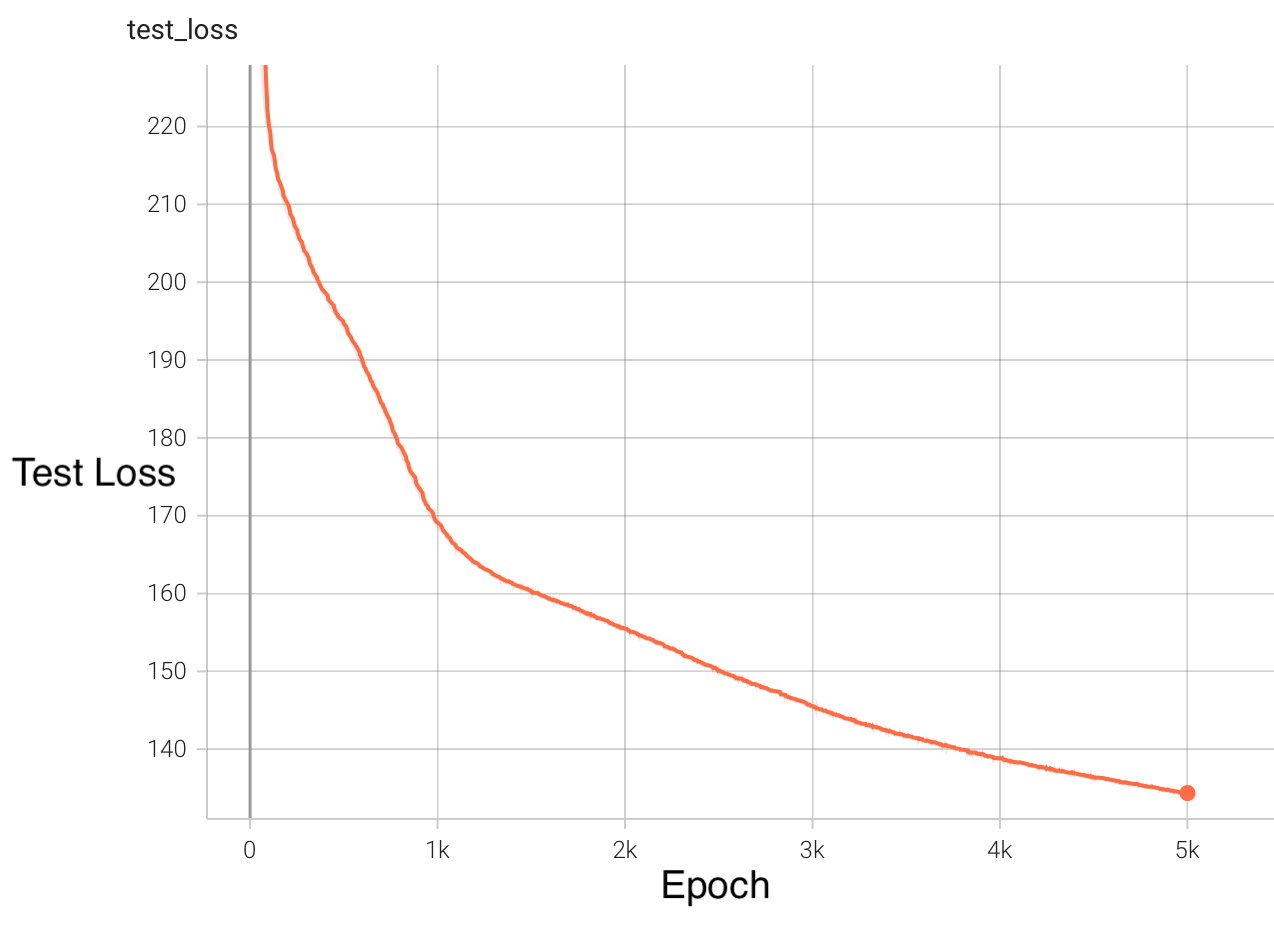
\includegraphics[scale=0.5]{circular_conv_test_loss.png}

After 5000 epochs of training, the train and test loss were both still decreasing, so additional training time is likely to have produced an even better model.
Also due to this limitation, it is difficult to tell whether the circular convolutional flows would have produced a better model than the normalising flows in our main experiments. 
